\section{Anwendungsfälle}
In \autoref{fig:usecase} wird das Use Case Diagramm dargestellt, welches die Anwendungsfälle der Website darstellt.
Da das Backend und der Mikrocontroller keine direkte Interaktion mit dem User ermöglichen, werden sie hier nicht erfasst.\\
\begin{figure}[h]
    \centering
    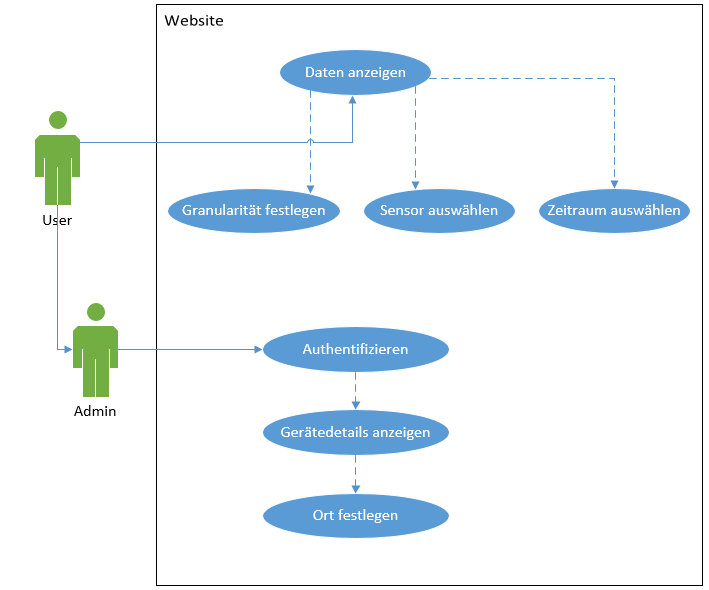
\includegraphics[width=0.7\linewidth]{img/usecase}
    \caption[Use Case Diagramm des Projekts]{Use Case Diagramm des Projekts (eigene Darstellung)}
    \label{fig:usecase}
\end{figure}

Der User hat auf der Website einen primären Anwendungsfall mit einigen Erweiterungen.
Neben der Anzeige der Daten kann der User die Granularität festlegen, also ändern wie viele Datenpunkte im Diagramm angezeigt werden.
Außerdem kann ein anderer Sensor aus dem Dropdown ausgewählt werden, um dessen Messwerte darzustellen.
%TODO sog. Daterangepicker erklären
Über den sogenannten \enquote{Daterangepicker} kann der Zeitraum festgelegt werden, in dem die Messdaten angezeigt werden. \\
Der Administrator hat neben den Anwendungsfällen des Users zusätzlich die Möglichkeit sich mit Nutzernamen und Passwort zu authentifizieren um das Administrator-Interface anzuzeigen.
Dort sind Gerätedetails aufgeführt und der Administrator kann den Standort des Sensors festlegen.